\documentclass[a4paper,12pt]{article}

%%% Работа с русским языком
\usepackage{cmap}					% поиск в PDF
\usepackage{mathtext} 				% русские буквы в формулах
\usepackage[T2A]{fontenc}			% кодировка
\usepackage[utf8]{inputenc}			% кодировка исходного текста
\usepackage[english,russian]{babel}	% локализация и переносы
\usepackage{xcolor}
\usepackage{hyperref}
 % Цвета для гиперссылок
\definecolor{linkcolor}{HTML}{799B03} % цвет ссылок
\definecolor{urlcolor}{HTML}{799B03} % цвет гиперссылок

\hypersetup{pdfstartview=FitH,  linkcolor=linkcolor,urlcolor=urlcolor, colorlinks=true}

%%% Дополнительная работа с математикой
\usepackage{amsfonts,amssymb,amsthm,mathtools} % AMS
\usepackage{amsmath}
\usepackage{icomma} % "Умная" запятая: $0,2$ --- число, $0, 2$ --- перечисление

%% Номера формул
%\mathtoolsset{showonlyrefs=true} % Показывать номера только у тех формул, на которые есть \eqref{} в тексте.

%% Шрифты
\usepackage{euscript}	 % Шрифт Евклид
\usepackage{mathrsfs} % Красивый матшрифт

%% Свои команды
\DeclareMathOperator{\sgn}{\mathop{sgn}}

%% Перенос знаков в формулах (по Львовскому)
\newcommand*{\hm}[1]{#1\nobreak\discretionary{}
{\hbox{$\mathsurround=0pt #1$}}{}}
% графика
\usepackage{graphicx}
\graphicspath{{pictures/}}
\DeclareGraphicsExtensions{.pdf,.png,.jpg}





\author{Бурмашев Григорий}
\title{Дискра - 2}
\date{\today}
\begin{document}
\begin{center}
Бурмашев Гриша. 208. Дискра-2
\end{center}
Пускай (для упрощения написания):
\[
x \in A = a\]
\[
x \in B = b
\]
\[
x \in C = c
\]
\section*{1}
Верно ли,  что для любых множеств A и B выполняется равенство:\\
\[
(A \setminus B) \cap ((A\cup B) \setminus (A \cap B)) = A \setminus B
\]
Выражение эквивалентно записи:
\[
(a \wedge \neg b) \wedge (a \vee b)\wedge \neg ( a \wedge b) = a \wedge \neg b
\]
Построим таблицу истинности для a, b:\\\\
\begin{tabular}{|c|c|c|c|c|c|c|}
\hline
 a&  b& $\neg$ b & $a \vee b$ & $\neg(a\wedge b) $& $a \wedge \neg b$ & $(a \wedge \neg b) \wedge (a \vee b)\wedge \neg ( a \wedge b)$\\
\hline
 0& 0 &1  &  0& 1 &  0 & 0\\
\hline
 0& 1 & 0 &  1& 1 &  0 & 0 \\
\hline
1 & 0 &1  & 1 &  1& 1 & 1\\
\hline
1 &1  & 0 & 1 &  0&  0 & 0 \\
\hline
\end{tabular}\\\\
Из таблицы (столбцы 6 и 7) видно, что равенство выполняется\\\\
\textbf{Ответ:} да, верно
\section*{2}
Верно ли,  что для любых множеств A, B, C выполняется равенство:\\
\[
(A \cap B) \setminus C = (A \setminus C) \cap (B \setminus C)
\]
Выражение эквивалентно записи:
\[
(a \wedge b) \wedge \neg c = (a \wedge \neg c) \wedge (b \wedge \neg c)
\]
\[
a \wedge b \wedge \neg c = a \wedge \neg c \wedge b \wedge \neg c
\]
Избавимся от повторения:
\[
a \wedge b \wedge \neg c = a \wedge b \wedge \neg c
\]
Выражения абсолютно эквивалентны\\\\
\textbf{Ответ:} да, верно
\section*{3}
Верно ли, что для любых множеств A и B выполняется включение:
\[
(A \cup B) \setminus (A \setminus B) \subseteq B
\]
Рассмотрим левую часть выражения:

Она эквивалентна записи:
\[
(a \vee b) \wedge \neg (a\wedge \neg b))
\]
Упростим и вынесем за скобки \textbf{b}:
\[
(a \vee b) \wedge (\neg a \vee b)
\]
\[
b \vee (a \wedge \neg a)
\]
$ a \wedge \neg a = 0$:
\[
b \vee 0 = b
\]
Таким образом:
\[
B \subseteq B
\]
Это верно\\\\
\textbf{Ответ:} да, верно
 \section*{4} 
Верно ли, что для любых множеств A, B и C выполняется равенство:
\[
((A \setminus B) \cup (A \setminus C)) \cap (A \setminus (B \cap C)) = A \setminus (B \cup C)
\]
Выражение эквивалетно записи:
\[
((a \wedge \neg b) \vee (a \wedge \neg c)) \wedge (a \wedge \neg (b \wedge c)) = a \wedge \neg (b \vee c)
\]
Вынесем \textbf{a} за скобку:
\[
(a \wedge (\neg b \vee \neg c)) \wedge ( a \wedge \neg(b \wedge c)) = a \wedge \neg (b \vee c)
\]
\[
(a \wedge (\neg b \vee \neg c)) \wedge ( a \wedge (\neg b \vee \neg c)) = a \wedge  (\neg b \wedge \neg  c)
\]
Избавимся от повторения:
\[
a \wedge (\neg b \vee \neg c) = a \wedge (\neg b \wedge \neg c)
\]
Выражения не равны

Пусть, например:
\[ a = 1\]
\[b = 0\]
\[c = 1\]
Тогда:
\[ 1 \wedge (1 \vee 0) = 1 \wedge (1 \wedge 0)
\]
\[
1 = 0
\]
Мы видим противоречие, значит, исходное равенство не выполняется\\\\
\textbf{Ответ:} нет, неверно
\section*{5}
Пусть $A_1 \supseteq A_2 \supseteq A_3 \supseteq \ldots  $ - невозрастающая последовательность множеств. Известно, что
$A_1 \setminus A_4  = A_6 \setminus A_9 $ 

Докажите, что $A_2 \setminus A_7 = A_3 \setminus A_8 $
\\\\
Представим $A_1 \setminus A_4 $ в виде:
\[
A_1 \setminus A_4 = A_1 \setminus A_2 + A_2 \setminus A_3 + A_3 \setminus A_4
\]
Это истинно, так как это эквивалентно:
\[
A_1 \wedge \neg A_4 = A_1 \wedge \neg A_2 \vee A_2 \wedge \neg A_3 \vee A_3 \wedge \neg A_4
\]
Упрощая:
\[
A_1 \wedge \neg A_4 = \neg A_1 \vee A_2 \vee \neg A_2 \vee A_3 \vee \neg A_3 \vee A_4
\]
\[
A_1 \wedge \neg A_4 = \neg A_1 \vee A_4
\]
\[
A_1 \wedge \neg A_4 = A_1 \wedge \neg A_4
\]
\begin{center}
Верно
\end{center}
В таком случае : 
\[
A_6 \setminus A_9 = A_6 \setminus A_7 + A_7 \setminus A_8 + A_8 \setminus A_9
\]
По условию, они равны друг другу, т.е:
\[
A_1 \setminus A_2 + A_2 \setminus A_3 + A_3 \setminus A_4 = A_6 \setminus A_7 + A_7 \setminus A_8 + A_8 \setminus A_9
\]
А так же по условию:
\[
A_1 \supseteq A_2 \supseteq A_3 \supseteq \ldots  \supseteq A_n \supseteq A_{n+1} \supseteq \ldots
\]
Т.е:
\[
A_1 \setminus A_4 \supseteq A_6 \setminus A_9
\]
При этом же мы знаем, что:
\[
A_1 \setminus A_4 = A_6 \setminus A_9
\]
Это возможно лишь в том случае, если:
\begin{equation}\label{1)}
A_1 \setminus A_2 + A_2 \setminus A_3 + A_3 \setminus A_4 = A_6 \setminus A_7 + A_7 \setminus A_8 + A_8 \setminus A_9 = \varnothing
\end{equation}
По аналогии:
\[
A_2 \setminus A_7 = A_2 \setminus A_3 + A_3 \setminus A_4 + \ldots + A_6 \setminus A_7
\]
\[
A_3 \setminus A_8 = A_3 \setminus A_4 + A_4 \setminus A_5 + \ldots + A_7 \setminus A_8
\]
Но из \ref{1)} :
\[
A_2 \setminus A_7 = \varnothing + \varnothing + A_4 \setminus A_5 + \varnothing
\]
\[
A_3 \setminus A_8 = \varnothing + A_4 \setminus A_5 + \varnothing + \varnothing 
\]
Т.е:
\[
A_2 \setminus A_7 = A_4 \setminus A_5 = A_3 \setminus A_8
\]
\[
A_2 \setminus A_7 = A_3 \setminus A_8
\]
\begin{center}
\textbf{Ч.Т.Д}
\end{center}
\section*{6}
Для любого целого положительного $n$ докажите равенство:
\[
1\times(n-1) + 2\times(n-2) + \ldots + (n-1)\times1 = \frac{(n-1)n(n+1)}{6}
\]
\begin{center}
Воспользуемся методом математической индукции:
\end{center}
\begin{itemize}
\item База:  n = 1
\[
1 \times 0 = \frac{0\times1\times2}{6}
\]
\[
0 = 0 
\]
\begin{center}
Верно
\end{center}
\item Переход: пусть верно для $n$, докажем, что это верно для $n=1$:
\[
1 \times n + 2\times(n-1) +\ldots + n \times 1 = \frac{n(n+1)(n+2)}{6}
\]
Если из новой последовательности вычесть изначальную, то мы получим:
\[
1 \times n + 2\times(n-1) +\ldots + n \times 1 - (1\times(n-1) + 2\times(n-2) + \ldots + (n-1)\times1)=
\]
\[
=n + 2n - 2 + \ldots n - n + 1 + -2n +4 - \ldots n + 1
\]
"n-ки" сокращаются и равенство превращается в:
\[
1 + 2 + 3 + \ldots + n
\]
\\
Это равно по сумме арифметической прогрессии:
\[
\frac{n(n+1)}{2}
\]
Пусть:
\[
A = 1\times(n-1) + 2\times(n-2) + \ldots + (n-1)\times1 =\frac{(n-1)n(n+1)}{6}
\]
\[
B = 1 \times n + 2\times(n-1) +\ldots + n \times 1
\]
Представим $ B $ как $A + B - A$, где $(B-A)$ мы уже нашли (сумма арифм.прогресиии):
\[
\frac{(n-1)n(n+1)}{6} + \frac{n(n+1)}{2} = \frac{(n-1)n(n+1)}{6} + \frac{3n(n+1)}{6}=
\]
\[
= \frac{(n+1)(n(n-1)+3n))}{6} = \frac{(n+1)(n^2+2n)}{6} = 
\]
\[
= \frac{(n+1)n(n+2)}{6} = \frac{n(n+1)(n+2)}{6}
\]
Т.е:
\[
B = \frac{n(n+1)(n+2)}{6} = 
\]
\[
= 1 \times n + 2\times(n-1) +\ldots + n \times 1
\]
\begin{center}

\textbf{Ч.Т.Д}
\end{center}
\end{itemize}
\section*{7}
Докажите, что для любого $ n \geq 1 $ выполняется равенство:
\[
F_{n-1} \times F_{n+1} - F^2_{n} = (-1)^{n+1}
\]
\begin{center}
Воспользуемся методом математической индукции:
\end{center}
\begin{itemize}
\item База: n = 1
\[
1 \times 2 - 1^2 = (-1)^2
\]
\[
1 = 1
\]
\begin{center}
\textbf{Верно}
\end{center}
\item Переход:
Пусть верно для $n$, докажем, что это верно для $n+1$:
\[
F_n \times F_{n+2} - F^2_{n+1} = (-1)^{n+2}
\]
\[
F_n\times(F_{n+1} + F_n) - F^2_{n+1} = (-1)^{n+1} \times (-1)
\]
Представим $(-1)^{n+1}$ как наше изначальное равенство:
\[
F_n \times F_{n+1} + F^2_n - F^2_{n+1} = -1(F_{n-1}\times F_{n+1} - F^2_n)
\]
\[
F^2_n + F_n \times F_{n+1} - F^2_{n+1}+ F_{n-1}\times F_{n+1} - F^2_n = 0\]
\[
F_{n+1} \times (F_n + F_{n-1}) - F^2_{n+1} = 0
\]
\[
F^2_{n+1} - F^2_{n+1} = 0
\]
\[
0 = 0
\]
\end{itemize}
\begin{center}
\textbf{Ч.Т.Д}
\end{center}
\section*{8} 
Докажите для  любого $ n > 1 $ неравенство:
\[
\frac{1}{n+1} + \frac{1}{n+2} + \ldots  + \frac{1}{2n}  > \frac{13}{24}
\]
\begin{center}
Воспользуемся методом математической индукции:
\end{center}
\begin{itemize}
\item База: $ n = 2 $
\[
\frac{1}{3} + \frac{1}{4} > \frac{13}{24}
\]
\\
\[
\frac{7}{12} > \frac{13}{24}
\]
\\
\[
\frac{14}{24} > \frac{13}{24}
\]
\begin{center}
 \textbf{Верно}
\end{center}

\item Переход:
\end{itemize} 
Пусть верно для $n$, тогда докажем для $n+1$:
\[
\frac{1}{n+2} + \frac{1}{n+3} + 
\ldots + \frac{1}{2n} + \frac{1}{2n+1} + \frac{1}{2(n+1)} > \frac{13}{24}
\]
Пусть наша исходная сумма равна $S_n$, а новая - $S_{n+1}$ т.е:
\[
S_n = \frac{1}{n+1} + \frac{1}{n+2} + \ldots  + \frac{1}{2n}
\]
\[S_{n+1} = \frac{1}{n+2} + \frac{1}{n+3} + 
\ldots + \frac{1}{2n} + \frac{1}{2n+1} + \frac{1}{2(n+1)}\]
\\\\
Если добавить и вычесть из $S_{n+1}$ множитель $\frac{1}{n+1}$, то можно заметить $S_n$:
\[
\frac{1}{n+1} - \frac{1}{n+1} + \frac{1}{n+2} + \frac{1}{n+3} + 
\ldots + \frac{1}{2n} + \frac{1}{2n+1} + \frac{1}{2(n+1)} > \frac{13}{24}
\]
Это эквивалентно:
\[
S_n - \frac{1}{n+1} + \frac{1}{2n+1} + \frac{1}{2(n+1)} > \frac{13}{24}
\]
Упростим:
\[
S_n + \frac{-2 + 1}{2n+2} + \frac{1}{2n+1} > \frac{13}{24}
\]
\[
S_n + \frac{-1}{2n+1} + \frac{1}{2n+1} > \frac{13}{24}
\]
\[
S_n + \frac{-2n-1 + 2n+2}{(2n+2)(2n+1)} > \frac{13}{24}
\]
\[
S_n + \frac{1}{(2n+2)(2n+1)} > \frac{13}{24}
\]
Мы знаем, что:
\[
S_n > \frac{13}{24}\]
\[
\frac{1}{(2n+2)(2n+1)} > 0
\text{ ,т.к }  n > 1 \text{ по условию}
\]
Следовательно верно: 
\[
S_n + \frac{1}{(2n+2)(2n+1)} > \frac{13}{24}
\]
Это эквивалентно:
\[
S_{n+1} > \frac{13}{24}
\]
\begin{center}
\textbf{Ч.Т.Д}
\end{center}
\section*{9}
В прямоугольнике $3 \times n$ (три строки и $n$ столбцов ) стоят фишки трёх цветов, по $ n $ штук каждого цвета. Докажите, что можно переставить фишки в каждой строке так, чтобы в каждом столбце были фишки всех цветов.\\\\
\textbf{Стоит заметить, что всего у нас 3n фишек.}\\
\begin{center}
Воспользуемся методом математической индукции:
\end{center}
\begin{itemize}
\item База: n = 1

Мы имеем прямоугольник размера $3 \times 1 $ и 3 фишки трех разных цветов. Пусть у нас есть цвета $r, g, b$, тогда очевидный случай:\\\\
\begin{tabular}{|c|c|c|}
\hline
 $r$ & $g $ &  $ b $\\
\hline
\end{tabular}\\
\begin{center}
\textbf{Верно}
\end{center}

\item Переход:\\

Пусть верно для $n$. Т.е мы сможем переставить $3n$ фишек трех разных цветов таким образом, чтобы в произвольном прямоугольнике размера $3\times n$  в каждом столбце были фишки всех цветов.\\
\newpage
Докажем, что это выполняется для $n+1$:\\\\
Из условия у нас есть $3(n+1) = 3n + 3$ фишек. Переставим фишки таким образом, чтобы в последней $n+1$ строке было три фишки трех разных цветов. Тогда у нас останется $3n$ фишек и прямоугольник размером $3\times n$. Но, по предположению индукции, мы сможем переставить $3n$ фишек в прямоугольнике $3 \times n$, чтобы в каждом столбце были фишки всех цветов. Таким образом, у нас расставлены фишки в прямоугольнике $ 3 \times n $ по предположению индукции, а оставшиеся 3 фишки разных цветов стоят в последней строчке (по построению)

\end{itemize}

\begin{center}
Визуализация:\\
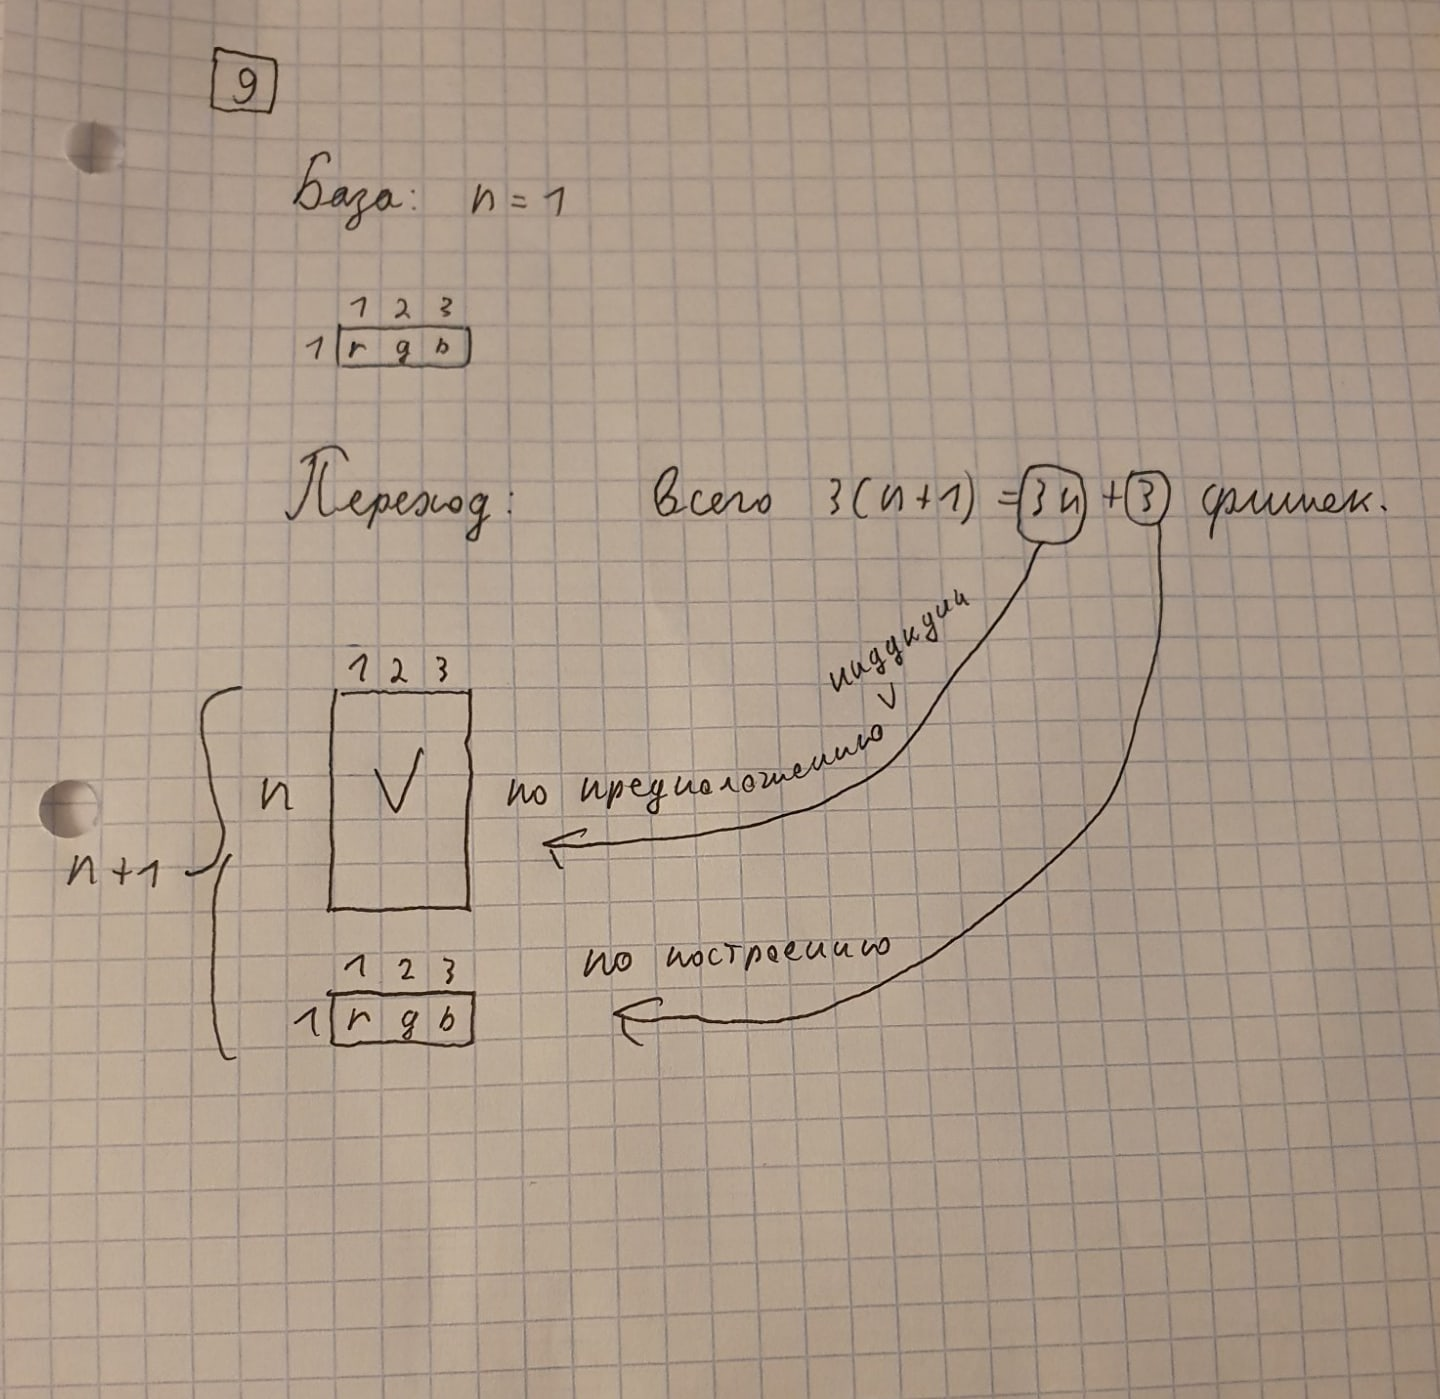
\includegraphics[scale=0.27]{9.jpg}
\end{center}
\begin{center}
\textbf{Ч.Т.Д}
\end{center}
\end{document}